\newpage
\newsection{Serverless Framework}
\subsection{Description}
The Serverless Framework is a free and open-source web framework written using Node.js. Serverless is the first framework that was originally developed for building applications exclusively on AWS Lambda, a serverless computing platform provided by Amazon as a part of the Amazon Web Services. Currently, applications developed with Serverless can be deployed to other function as a service providers, including Microsoft Azure with Azure Functions, IBM Bluemix with IBM Cloud Functions based on Apache OpenWhisk, Google Cloud using Google Cloud Functions, Oracle Cloud using Oracle Fn, Kubeless based on Kubernetes, Spotinst and Webtask by Auth0.

A Serverless app can simply be a couple of lambda functions to accomplish some tasks, or an entire back-end composed of hundreds of lambda functions. Serverless currently supports Node.js and Python runtime.

\subsection{Serverless.yml}
One advantage of using this tool is the capability to deploy every time an entire serverless system based on cloud providers, in this case AWS. You can define a \emph{serverless.yml} configuration file which contains all the informations about your service. You don't need to manually create the resources you need in a project, like database tables, queues, API endpoints and Lambda functions. You just have to write the code and then deploying your app.\\

Example of serverless.yml configuration for User Management:\\

\begin{itemize}
\begin{figure} [H]
\item Name of your services and list of plugins: the \emph{split-stack} plugin is useful when you reach the limit of 200 resources to deploy because it automatically split your resources using nested stacks;

	\centering
	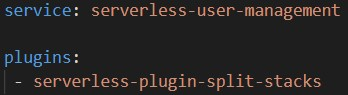
\includegraphics[scale=1.2]{../Img/serv1}
	\caption{Plugins - serverless.yml}\label{}
\end{figure}

\begin{figure} [H]
\item About your cloud provider: you can also define your IAM role authorization policies;

	\centering
	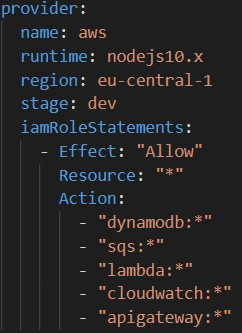
\includegraphics[scale=1.2]{../Img/serv2}
	\caption{Provider info - serverless.yml}\label{}
\end{figure}

\begin{figure} [H]
\item DynamoDB tables parameters: you have to define the name of the table, name and type of the key and the previsioned throughput;

	\centering
	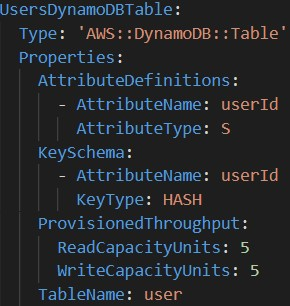
\includegraphics[scale=1.2]{../Img/serv3}
	\caption{DynamoDB tables - serverless.yml}\label{}
\end{figure}

\begin{figure} [H]
\item Lambda function and its handler: you can also define which events trigger that lambda. In this case the trigger event is when new object arrives into the specified queue; 

	\centering
	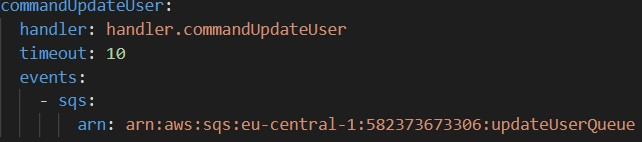
\includegraphics[scale=1.2]{../Img/serv4}
	\caption{Lambda triggered by SQS event - serverless.yml}\label{}
\end{figure}

\item You can define an API gateway endpoint which trigger the corresponding function: you can also use a custom request template.
\begin{figure} [H]
	\centering
	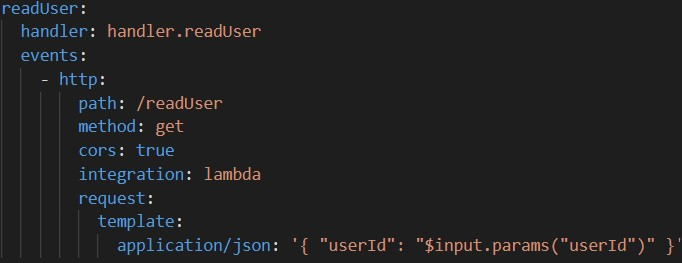
\includegraphics[scale=1.2]{../Img/serv5}
	\caption{Lambda triggered by GET endpoint - serverless.yml}\label{}
\end{figure}

\end{itemize}


\subsection{Project's root}
\begin{figure} [H]
The main project's handler is composed of the other handlers, one per aggregate and another one to handle event sourcing functions. In this way the responsibilities are restricted to every type of aggregate.

	\centering
	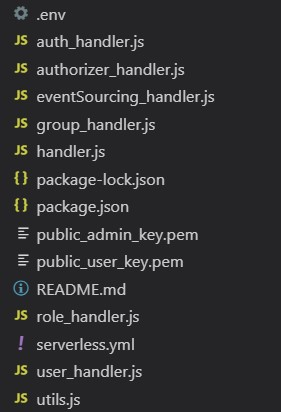
\includegraphics[scale=1.4]{../Img/root}
	\caption{Project's root}\label{}
\end{figure}
